\chapter{Progress}\label{progress}
\section{Rheology and Sliding Study}\label{study1}
Building upon the diagnostic ISMIP-HOM experiments in~\cite{Pattyn_2008}, I extend the prognostic experiment F to systematically investigate the combined effects of rheology and basal sliding within a benchmark ice sheet model. The original experiment F included two scenarios: one with a frozen bed (no-slip) and another with linear sliding.
My study expands upon these conditions by also incorporating non-linear rheology. This addition generates four distinct scenarios for comparison:
\begin{itemize}
\item{S1} No-slip (frozen) bed + Linear rheology ($n=1$).
\item{S2} No-slip (frozen) bed + Non-linear rheology ($n=4$).
\item{S3} Linear sliding + Linear rheology ($n=1$).
\item{S4} Linear sliding + Non-linear rheology ($n=4$).
\end{itemize}
While the original study by Pattyn et al. (2008) covered scenarios S1 and S3, understanding the impact of rheological assumptions is crucial for modern ice sheet modelling. During periods of rapid grounding line retreat, uncertainty in the Glen flow law exponent $n$ has been found to cause a larger spread in ice-loss projections than uncertainty in climate forcing~\cite{Getraer_2025}.

\subsection{Non-Linear Rheology for Exp F}
This rheology study directly addresses a critical gap in current inversion methods. While approaches like Ockenden et al. (2023) assume linear rheology ($n=1$), my results (see Figures~\ref{fig:elev_vel_S1_S2} and~\ref{fig:elev_vel_S3_S4}) demonstrate that non-linear rheology produces substantially different bed-to-surface transfer characteristics. These findings will enable BedSAT to incorporate rheology-dependent transfer functions, potentially improving bed topography reconstruction accuracy in regions where non-linear ice behavior dominates.
The method I follow to ensure that different model rheologies start from identical initial conditions is based on the re-scaling method by Getraer and Morlighem (2025)~\cite{Getraer_2025}. Their formula ensures that the initial ice viscosity—and therefore strain rates for a given stress—is identical between simulations with different rheologies.
For the non-linear scenarios I am considering $n = 4$, since the assumption of $n = 3$ for ice deformation is not universally supported and values of $n > 3$ have been inferred from real‐world glaciers. 
The resultant surface elevations and velocities after a 300 year transient evolution For the frozen and sliding bed scenarios are 
\begin{figure}[H]
    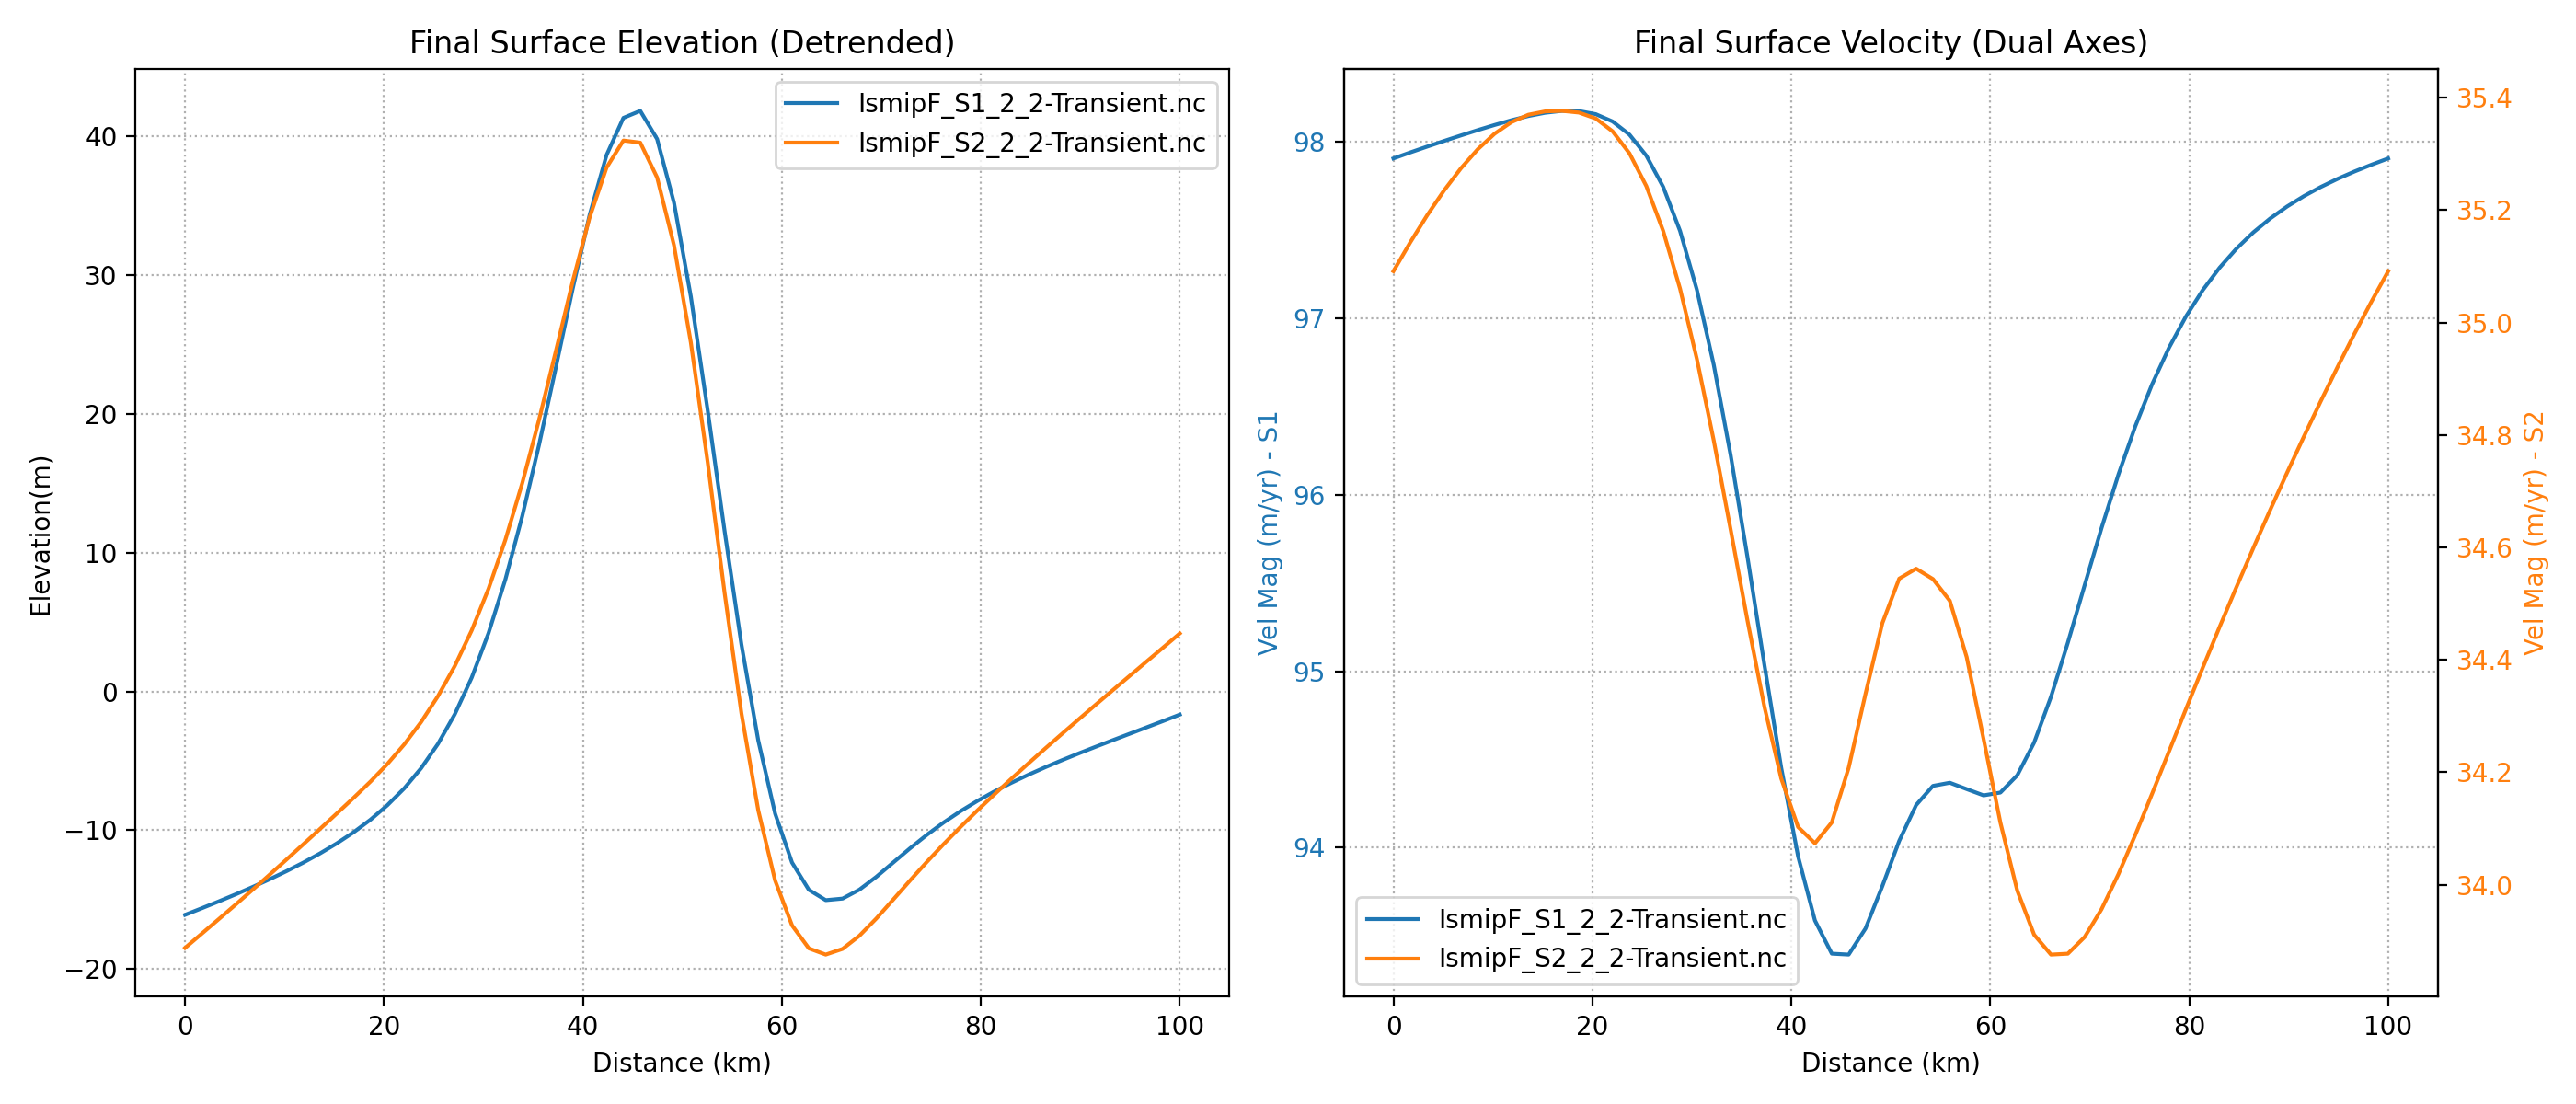
\includegraphics[scale=0.40]{figures/combined_elevation_detrended_surface_velocity_['S1']_['S2'].png}
    \caption{Final surface elevations and velocities for the original frozen bed Experiment F (S1) and the corresponding transformed to non-linear rheology experiment (S2)}
    \label{fig:elev_vel_S1_S2}
\end{figure}
\begin{figure}[H]
    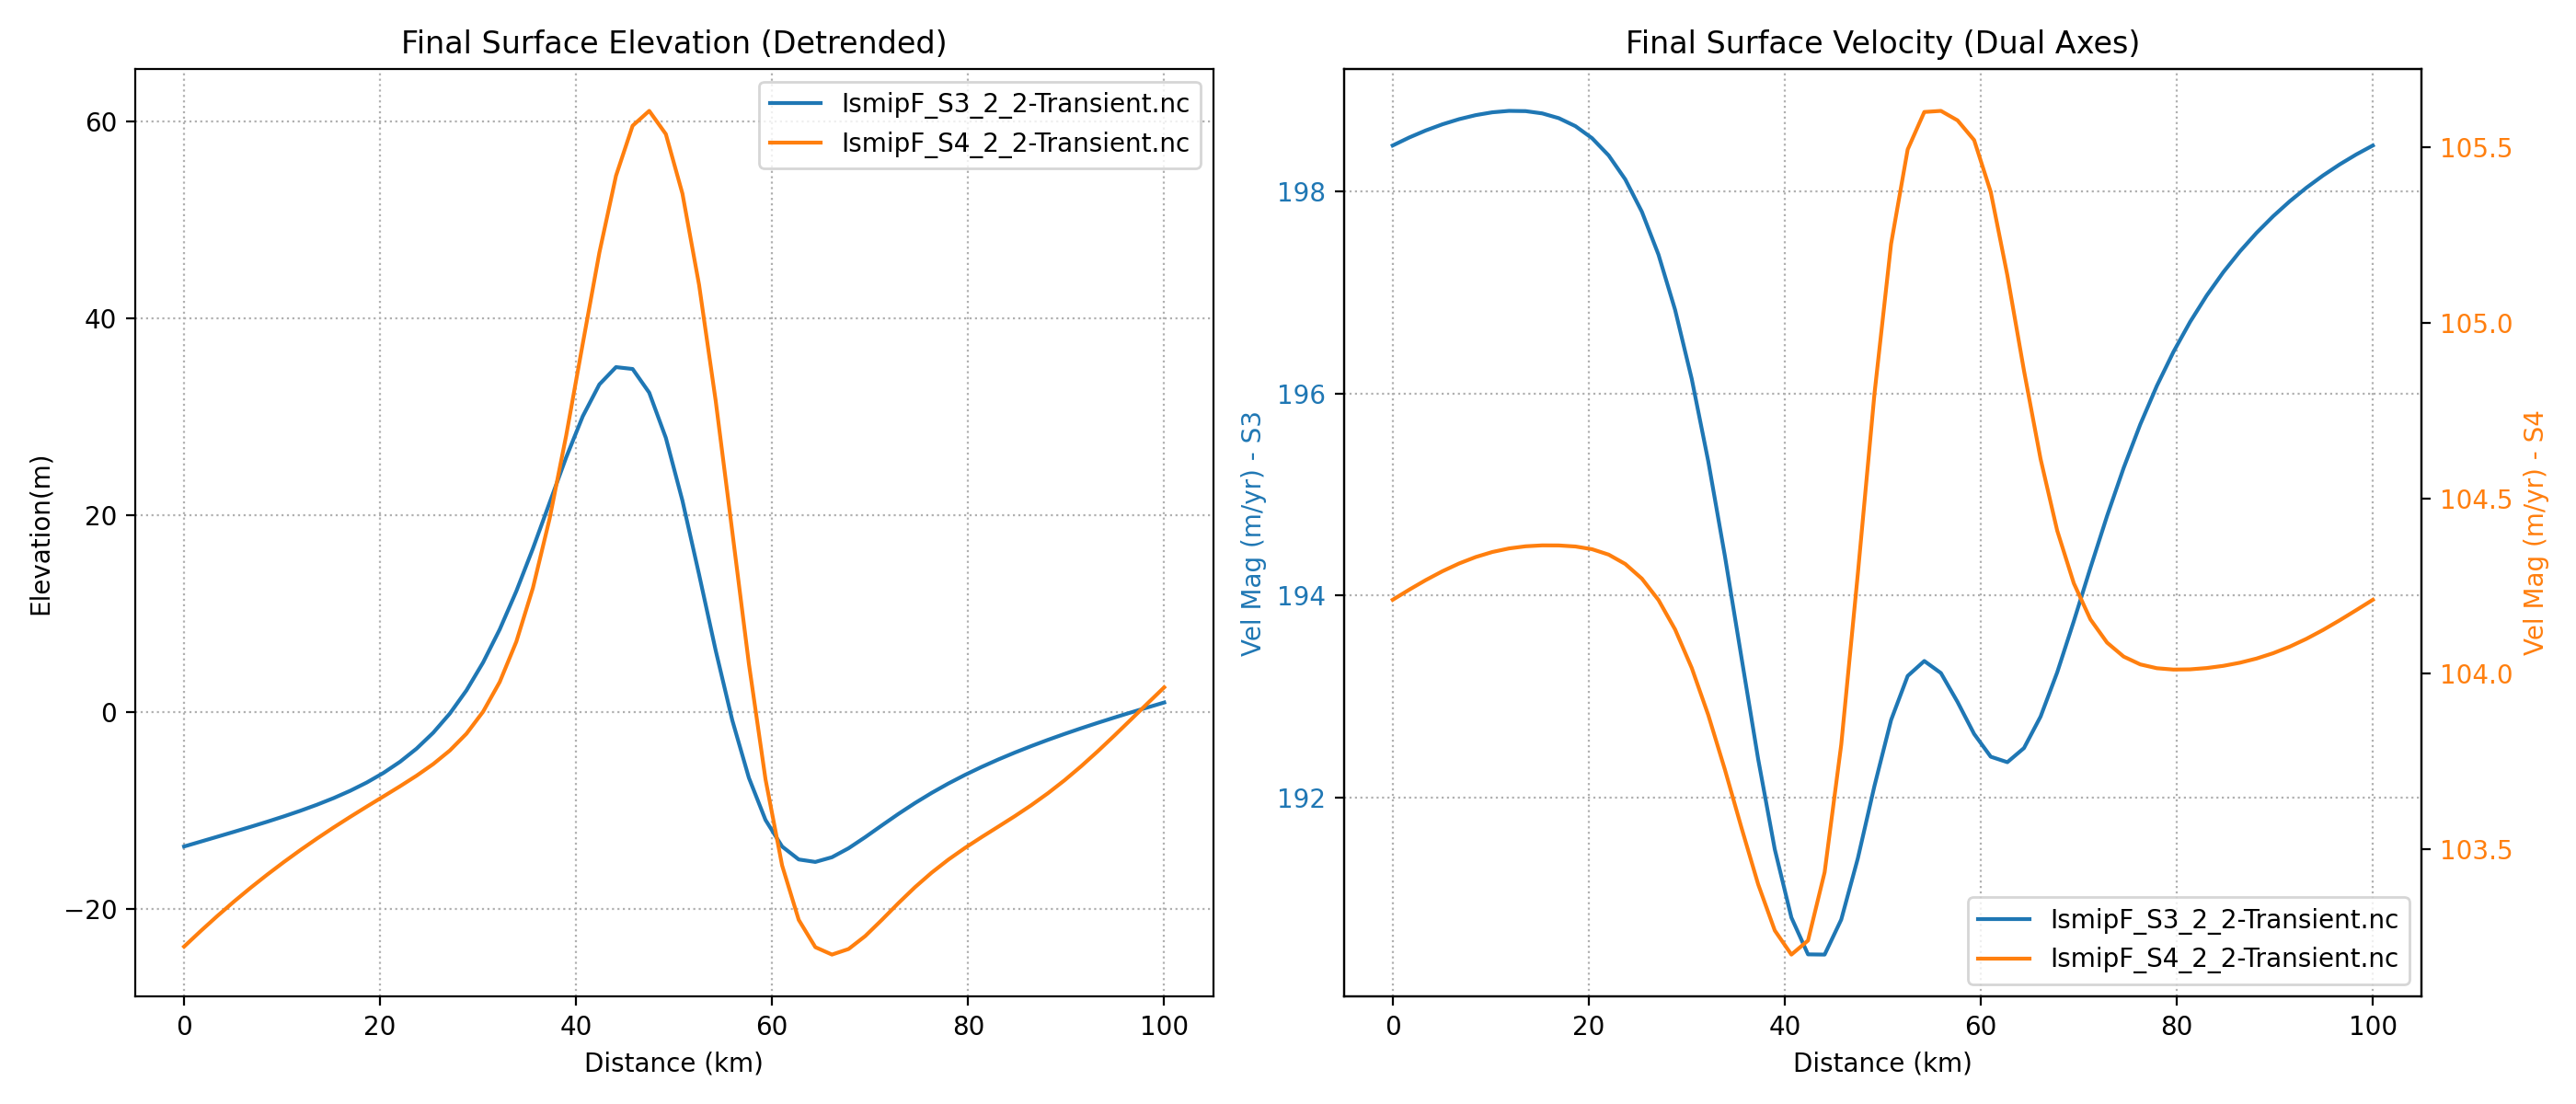
\includegraphics[scale=0.40]{figures/combined_elevation_detrended_surface_velocity_['S3']_['S4'].png}
    \caption{Final surface elevations and velocities for the original sliding bed Experiment F (S3) and the corresponding transformed to non-linear rheology experiment (S4)}
    \label{fig:elev_vel_S3_S4}
\end{figure}
The linear results results are consistent with the surface elevation and velocities found by Pattyn et al. (2008) for Exp. F—along the central flowline of the domain—for the both the frozen and sliding experiments. Meanwhile, the non-linear scenarios (S2 and S4) shown in orange in Figures~\ref{fig:elev_vel_S3_S4} and~\ref{fig:elev_vel_S1_S2} represent the first key finding of this analysis. The marked differences in both final surface elevation and velocity compared to the linear counterparts (S1, S3) provide crucial evidence for my first research question (``How does the bed topography manifest on the ice surface?''). The ice viscosity and hence its deformation is directly influenced by the stress and strain according to Glen's flow law. Given the power law relationship, using an $n = 4$ exponent leads to a strong non-linear relationship where a small increase in stress yields a much larger increase in deformation. This becomes visible as more complex flow adjustments—ice becomes softer in high stress regions and stiffer in low stress ones—in the non-linear models. These results demonstrate that the choice of rheology is not a minor parameter choice, but a control on the bed-to-surface signal transfer. This directly implies that a succesful inversion framework like BedSAT must account for non-linear effects, a limitation in some existing methods that assume a simpler linear rheology.
% Realistic rheology assumptions could theoretically produce surface patterns that better match satellite observations, potentially improving inversion accuracy. However, it is necessary to address that this study's aim is also to quantify whether this increased realism improves bed topography reconstruction accuracy enough to justify the additional computational complexity in the inversion framework. The next stage in this investigation is developing a variety of synthetic bedrock topographies to understand the relationship between basal geometry, ice rheology, and overall flow response to more complex bed conditions. This bedrock database will be used to create a large data set of bed features to surface (response) features that leverages the PhysicsNeMo-ML inference capabilities (see subsection~\ref{ML}).
\section{The Current Computational Framework of this Study}
This study is supported by a suite of interconnected scripts and tools designed for generating conditions, running simulations, processing output, and performing scientific analysis.
The core of this study is a time evolution flow simulation of fully grounded ice over 300 years with daily time steps. This simulation is designed to systematically investigate the relationship between basal geometry, ice rheology and flow response by running a series of ISMIP-HOM style experiments~\cite{Pattyn_2008} that can later be analysed in detail with other data processing tools~\ref{analysis_tools}. The simulations solve Higher order (HO) ice flow equations for a static diagnostic stress balance and a transient run (which includes stress balance and mass transport configurations).
\subsection{Data Processing, Visualization and Scientific Analysis Tools}\label{analysis_tools}
I have developed a set of robust, high-performance scripts to handle the large volume of data produced by the ice flow simulations. (Note that: All batch scripts have their individual file processing counterpart)
\begin{figure}[H]
    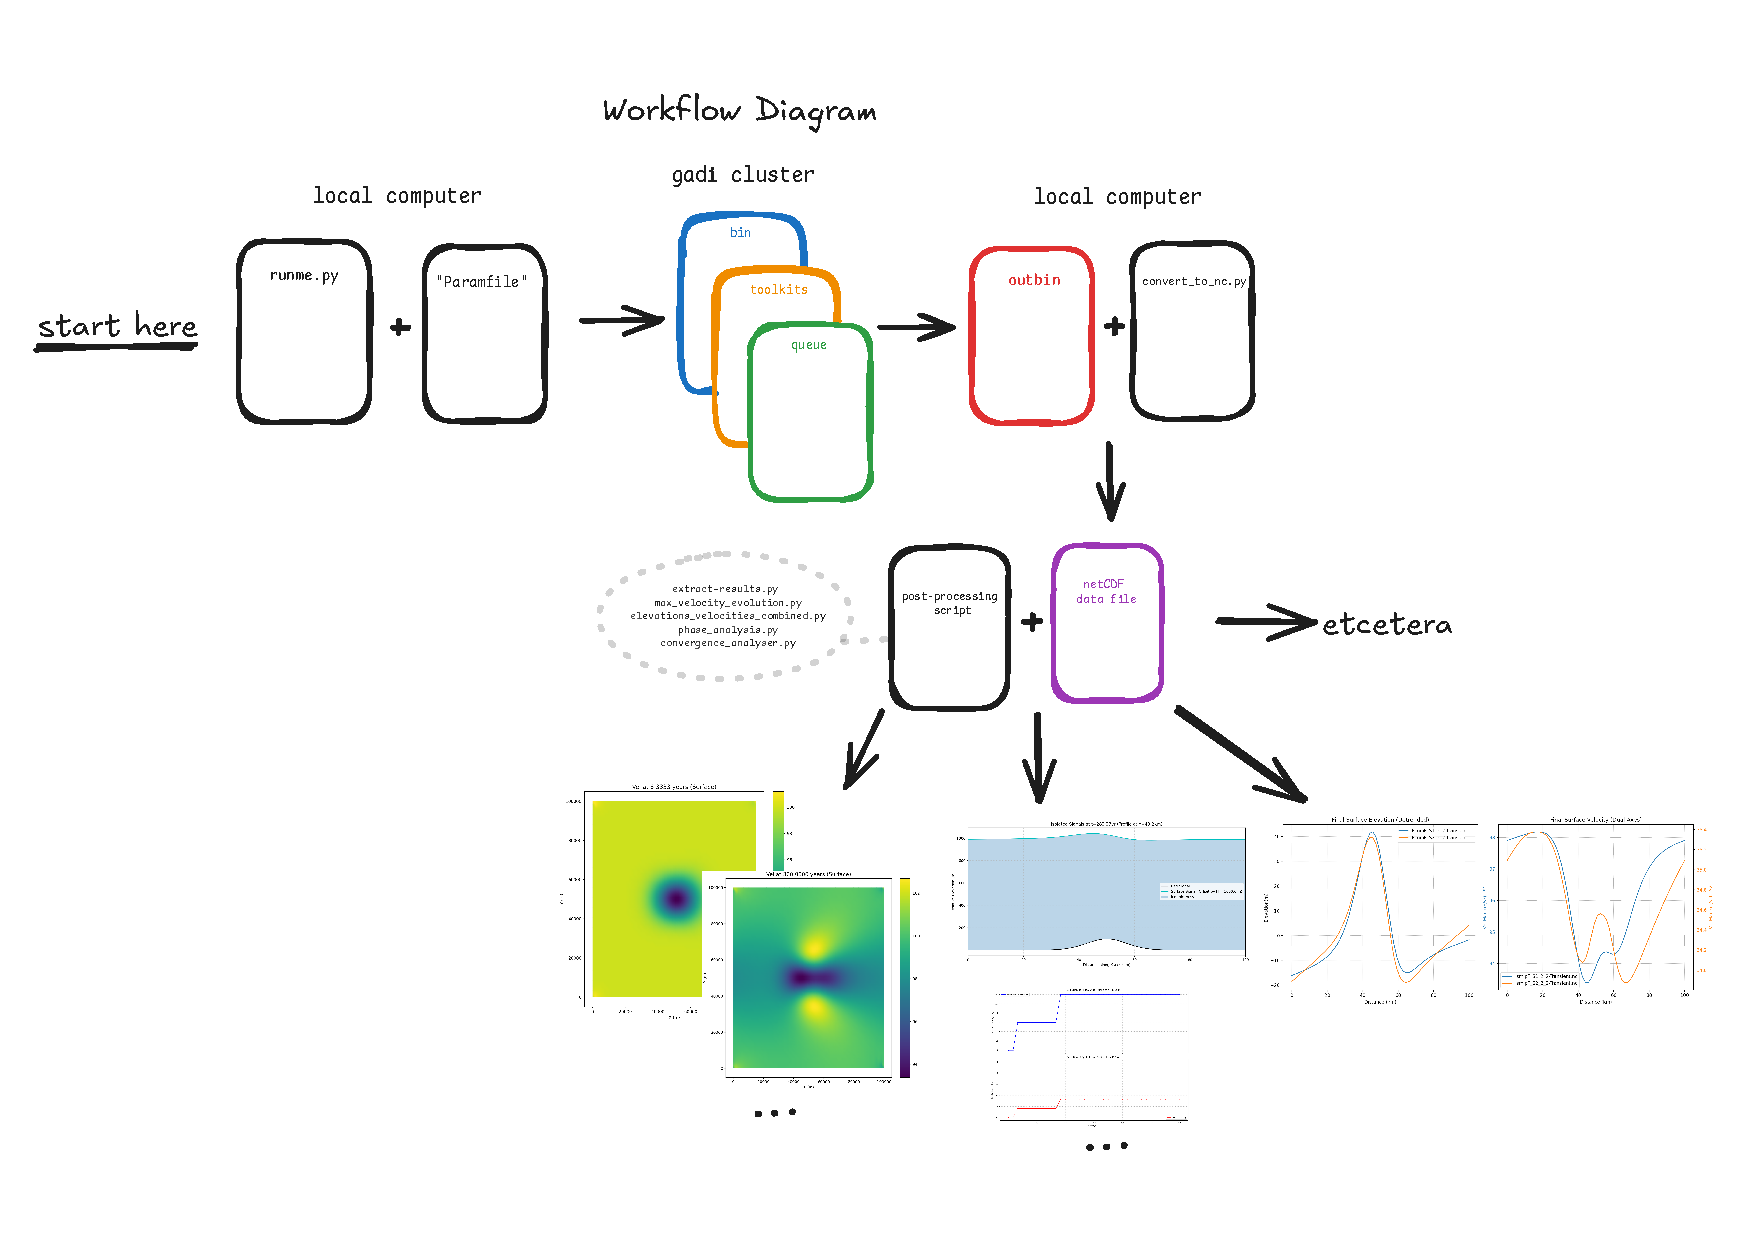
\includegraphics[scale=0.58]{figures/workflow_diagram.pdf}
    \caption{Diagrammatic representation of the current workflow using my ice simulation and analysis suite. For a particular simulation I will extract the results and visually inspect the output using  all analysis scripts in the suite.}\label{fig:workflow}
\end{figure}
\begin{enumerate}
\item{Binary to NetCDF Conversion} A batch-capable tool (\texttt{batch\_convert.py}) converts ISSM \texttt{.outbin} files into the standard, portable NetCDF format. This script supports parallel processing for high throughput.
\item{Result Extraction and Visualization} A batch script (\texttt{batch\_extract\_results.py}) that automatically finds and processes NetCDF files to generate visualisations of key fields like velocity and pressure. 
\item{Targeted Scientific Plotting} Additional scripts are used to create specific scientific plots.
\end{enumerate}
As per Figure~\ref{fig:workflow}, my workflow requires more automation. This is  a work in progress.
% \newpage
\subsubsection{Grid Independence}\label{grid_ind}
\begin{figure}[H]
    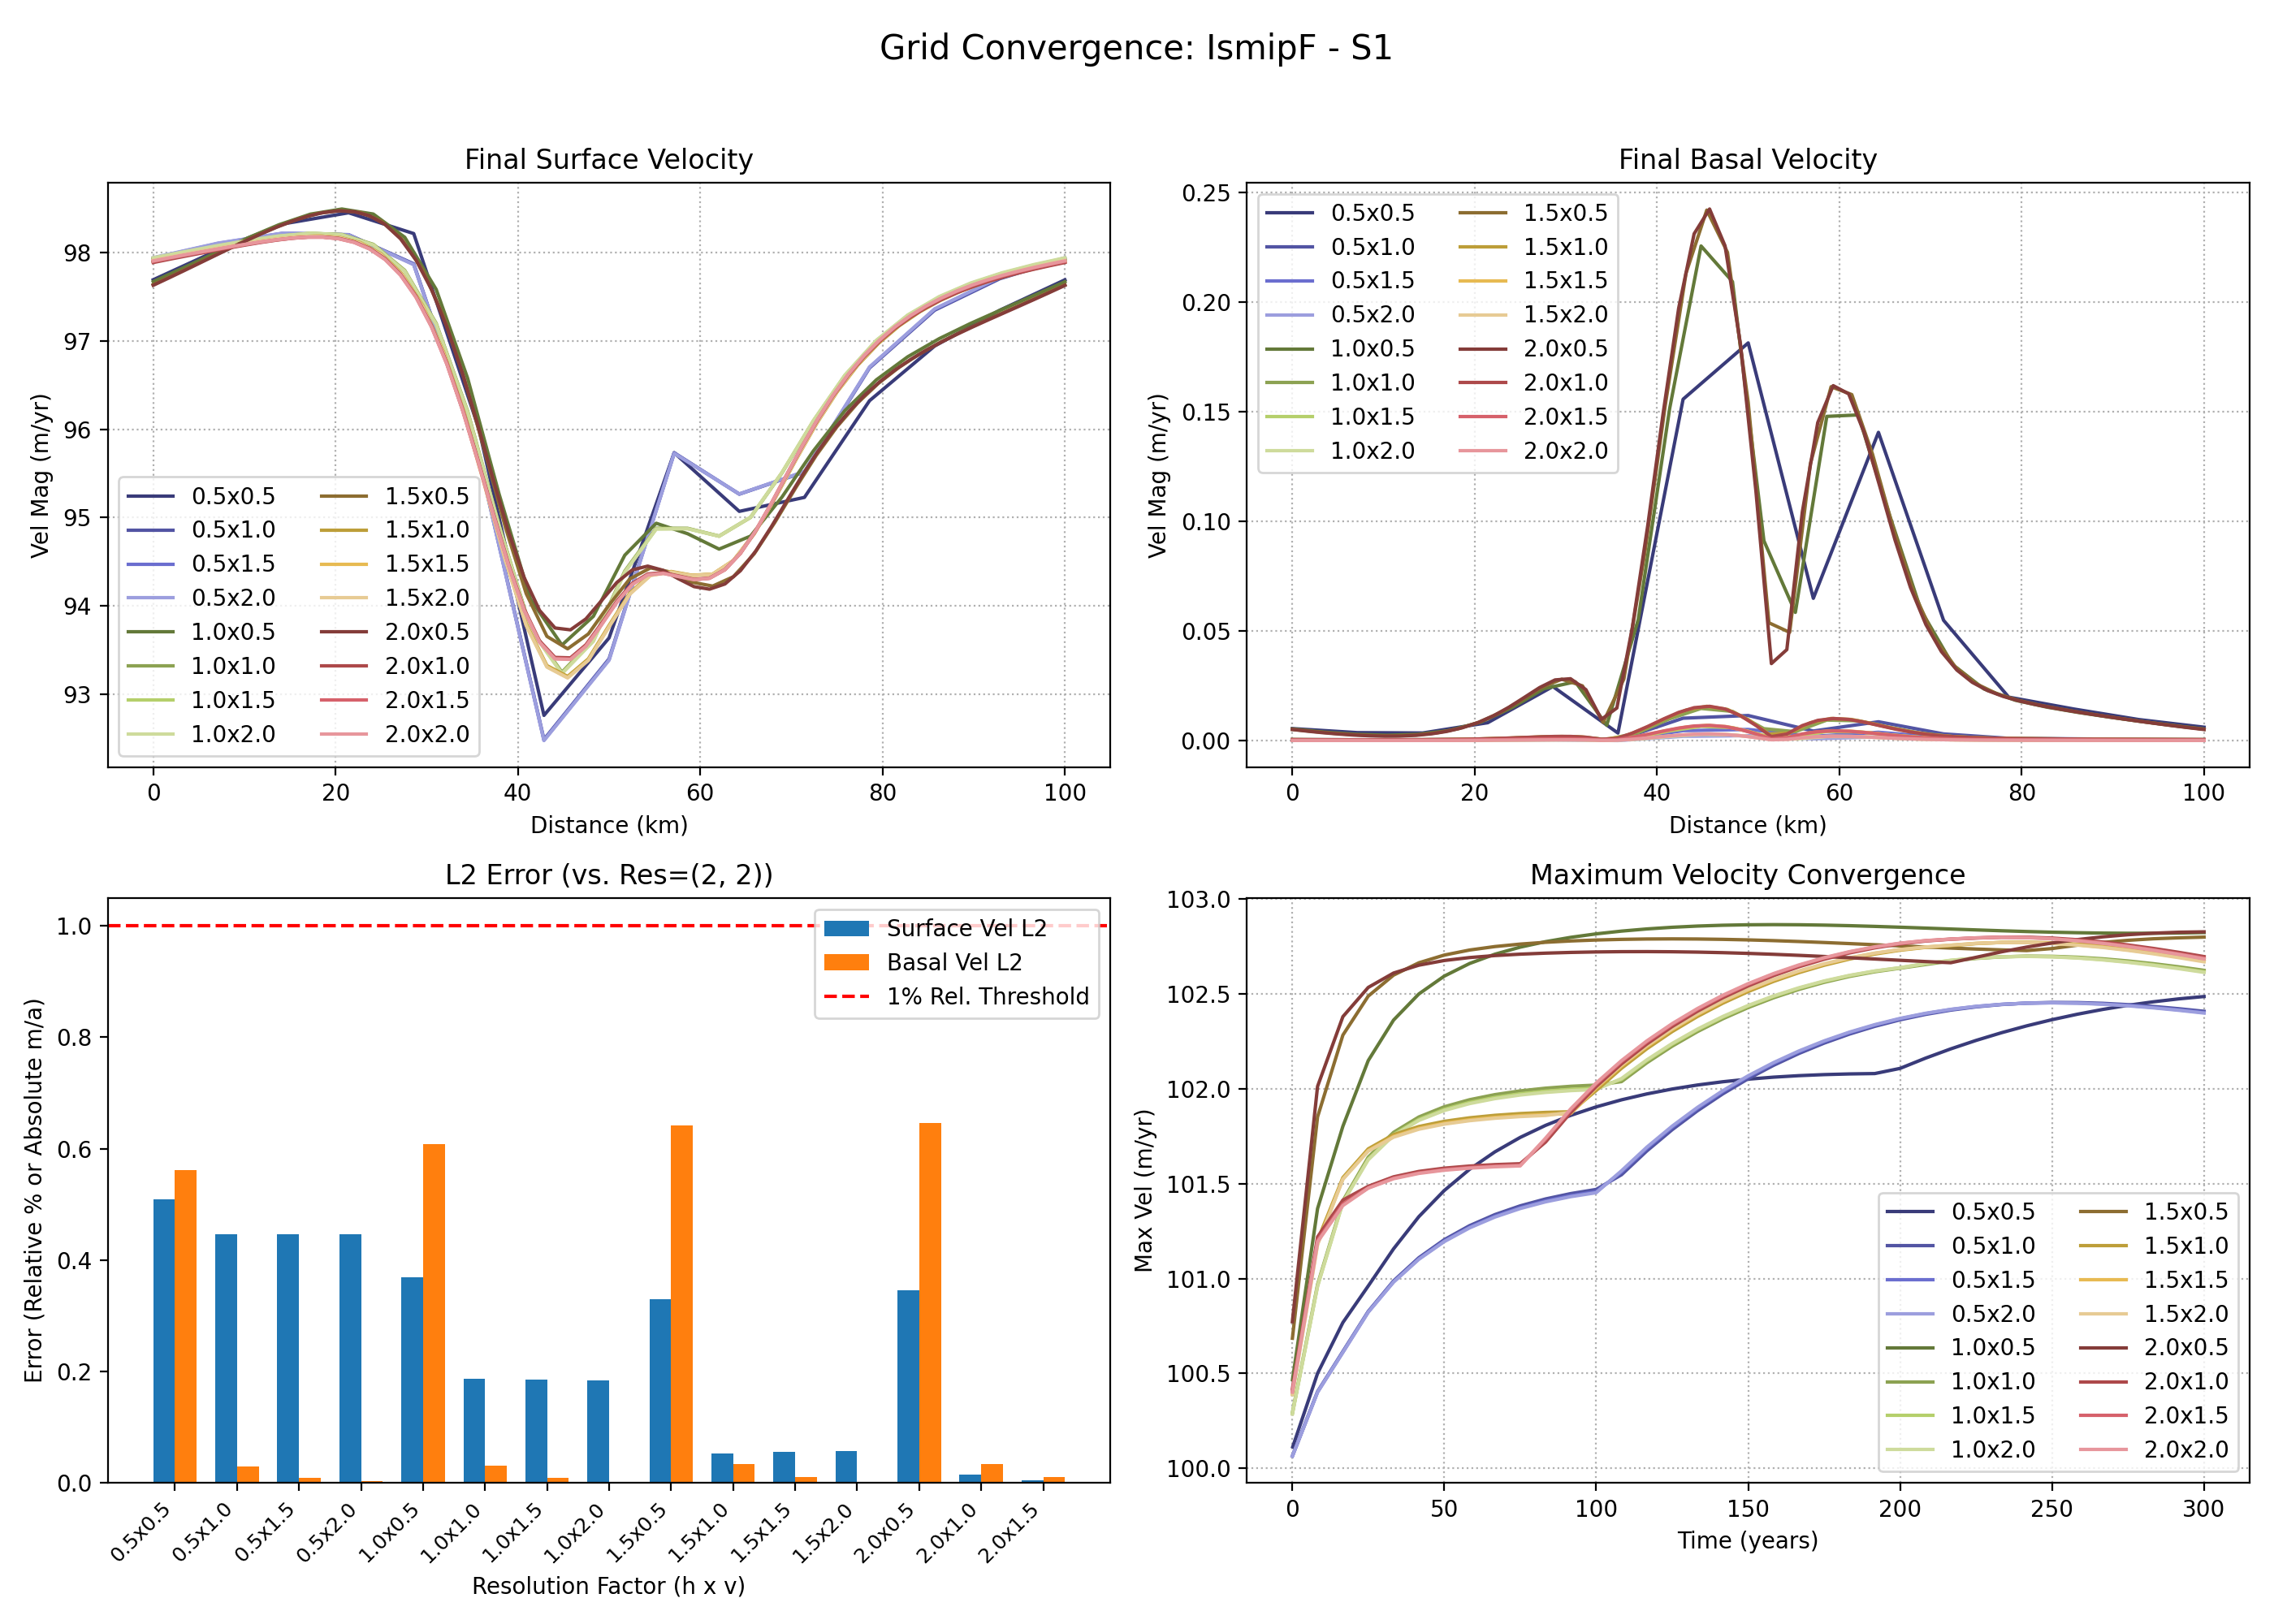
\includegraphics[scale=0.40]{figures/IsmipF_S1_convergence_summary.png}
    \caption{Grid convergence analysis for Scenario S1 (frozen bed, linear rheology, $n=1$). The four panels show: (top-left) final surface velocity profiles and (top-right) final basal velocity profiles for 16 different mesh resolutions; (bottom-left) the L2 relative error of each simulation compared to the highest-resolution mesh ($2.0\times2.0$), with a 1\% relative error threshold indicated by the dashed line; and (bottom-right) the evolution of the maximum velocity over the 300-year simulation period}
    \label{fig:grid_conv_S1}
\end{figure}
\begin{figure}[H]
    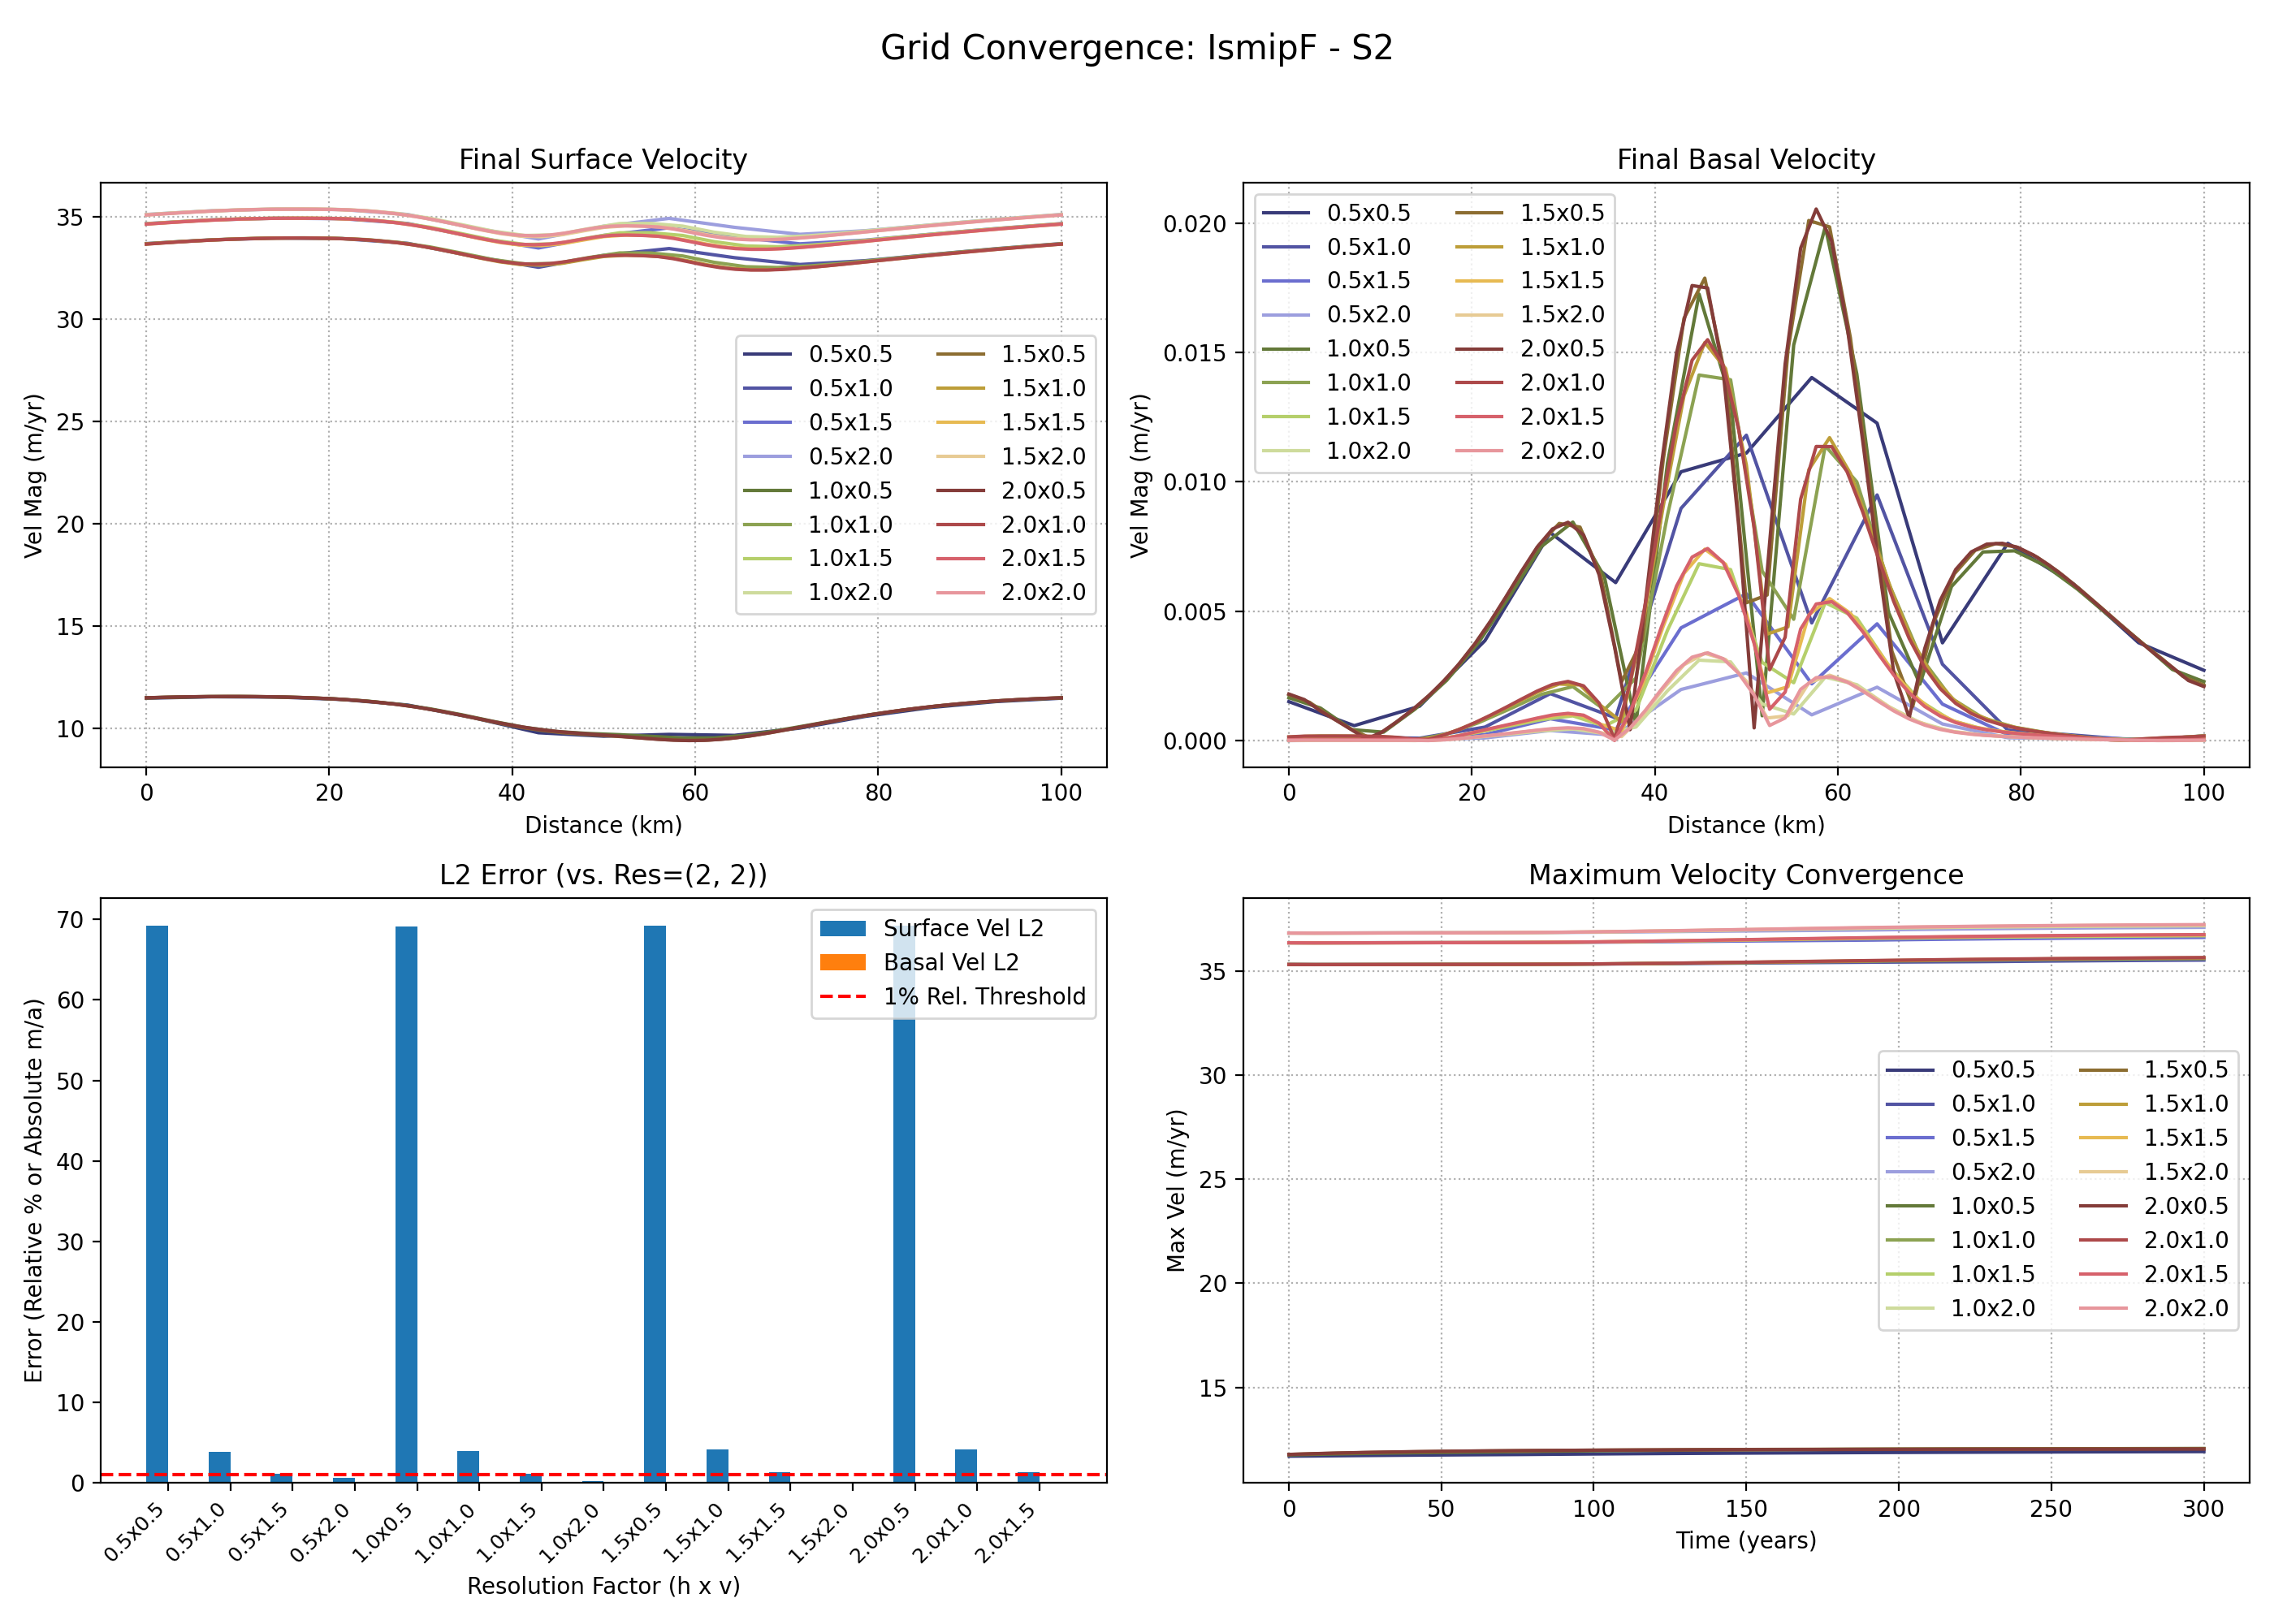
\includegraphics[scale=0.40]{figures/IsmipF_S2_convergence_summary.png}
    \caption{Grid convergence analysis for Scenario S2 (frozen bed, non-linear rheology, $n=4$). An extension of ISMIP-HOM Experiment F. The panels display the same metrics as Figure~\ref{fig:grid_conv_S1}. This scenario exhibits high sensitivity to vertical resolution refinement, with low-resolution simulations showing the highest errors and converging to a much slower flow state ($\approx~11$ m/a) compared to high-resolution runs ($\approx~37$ m/a).}
    \label{fig:grid_conv_S2}
\end{figure}
\begin{figure}[H]
    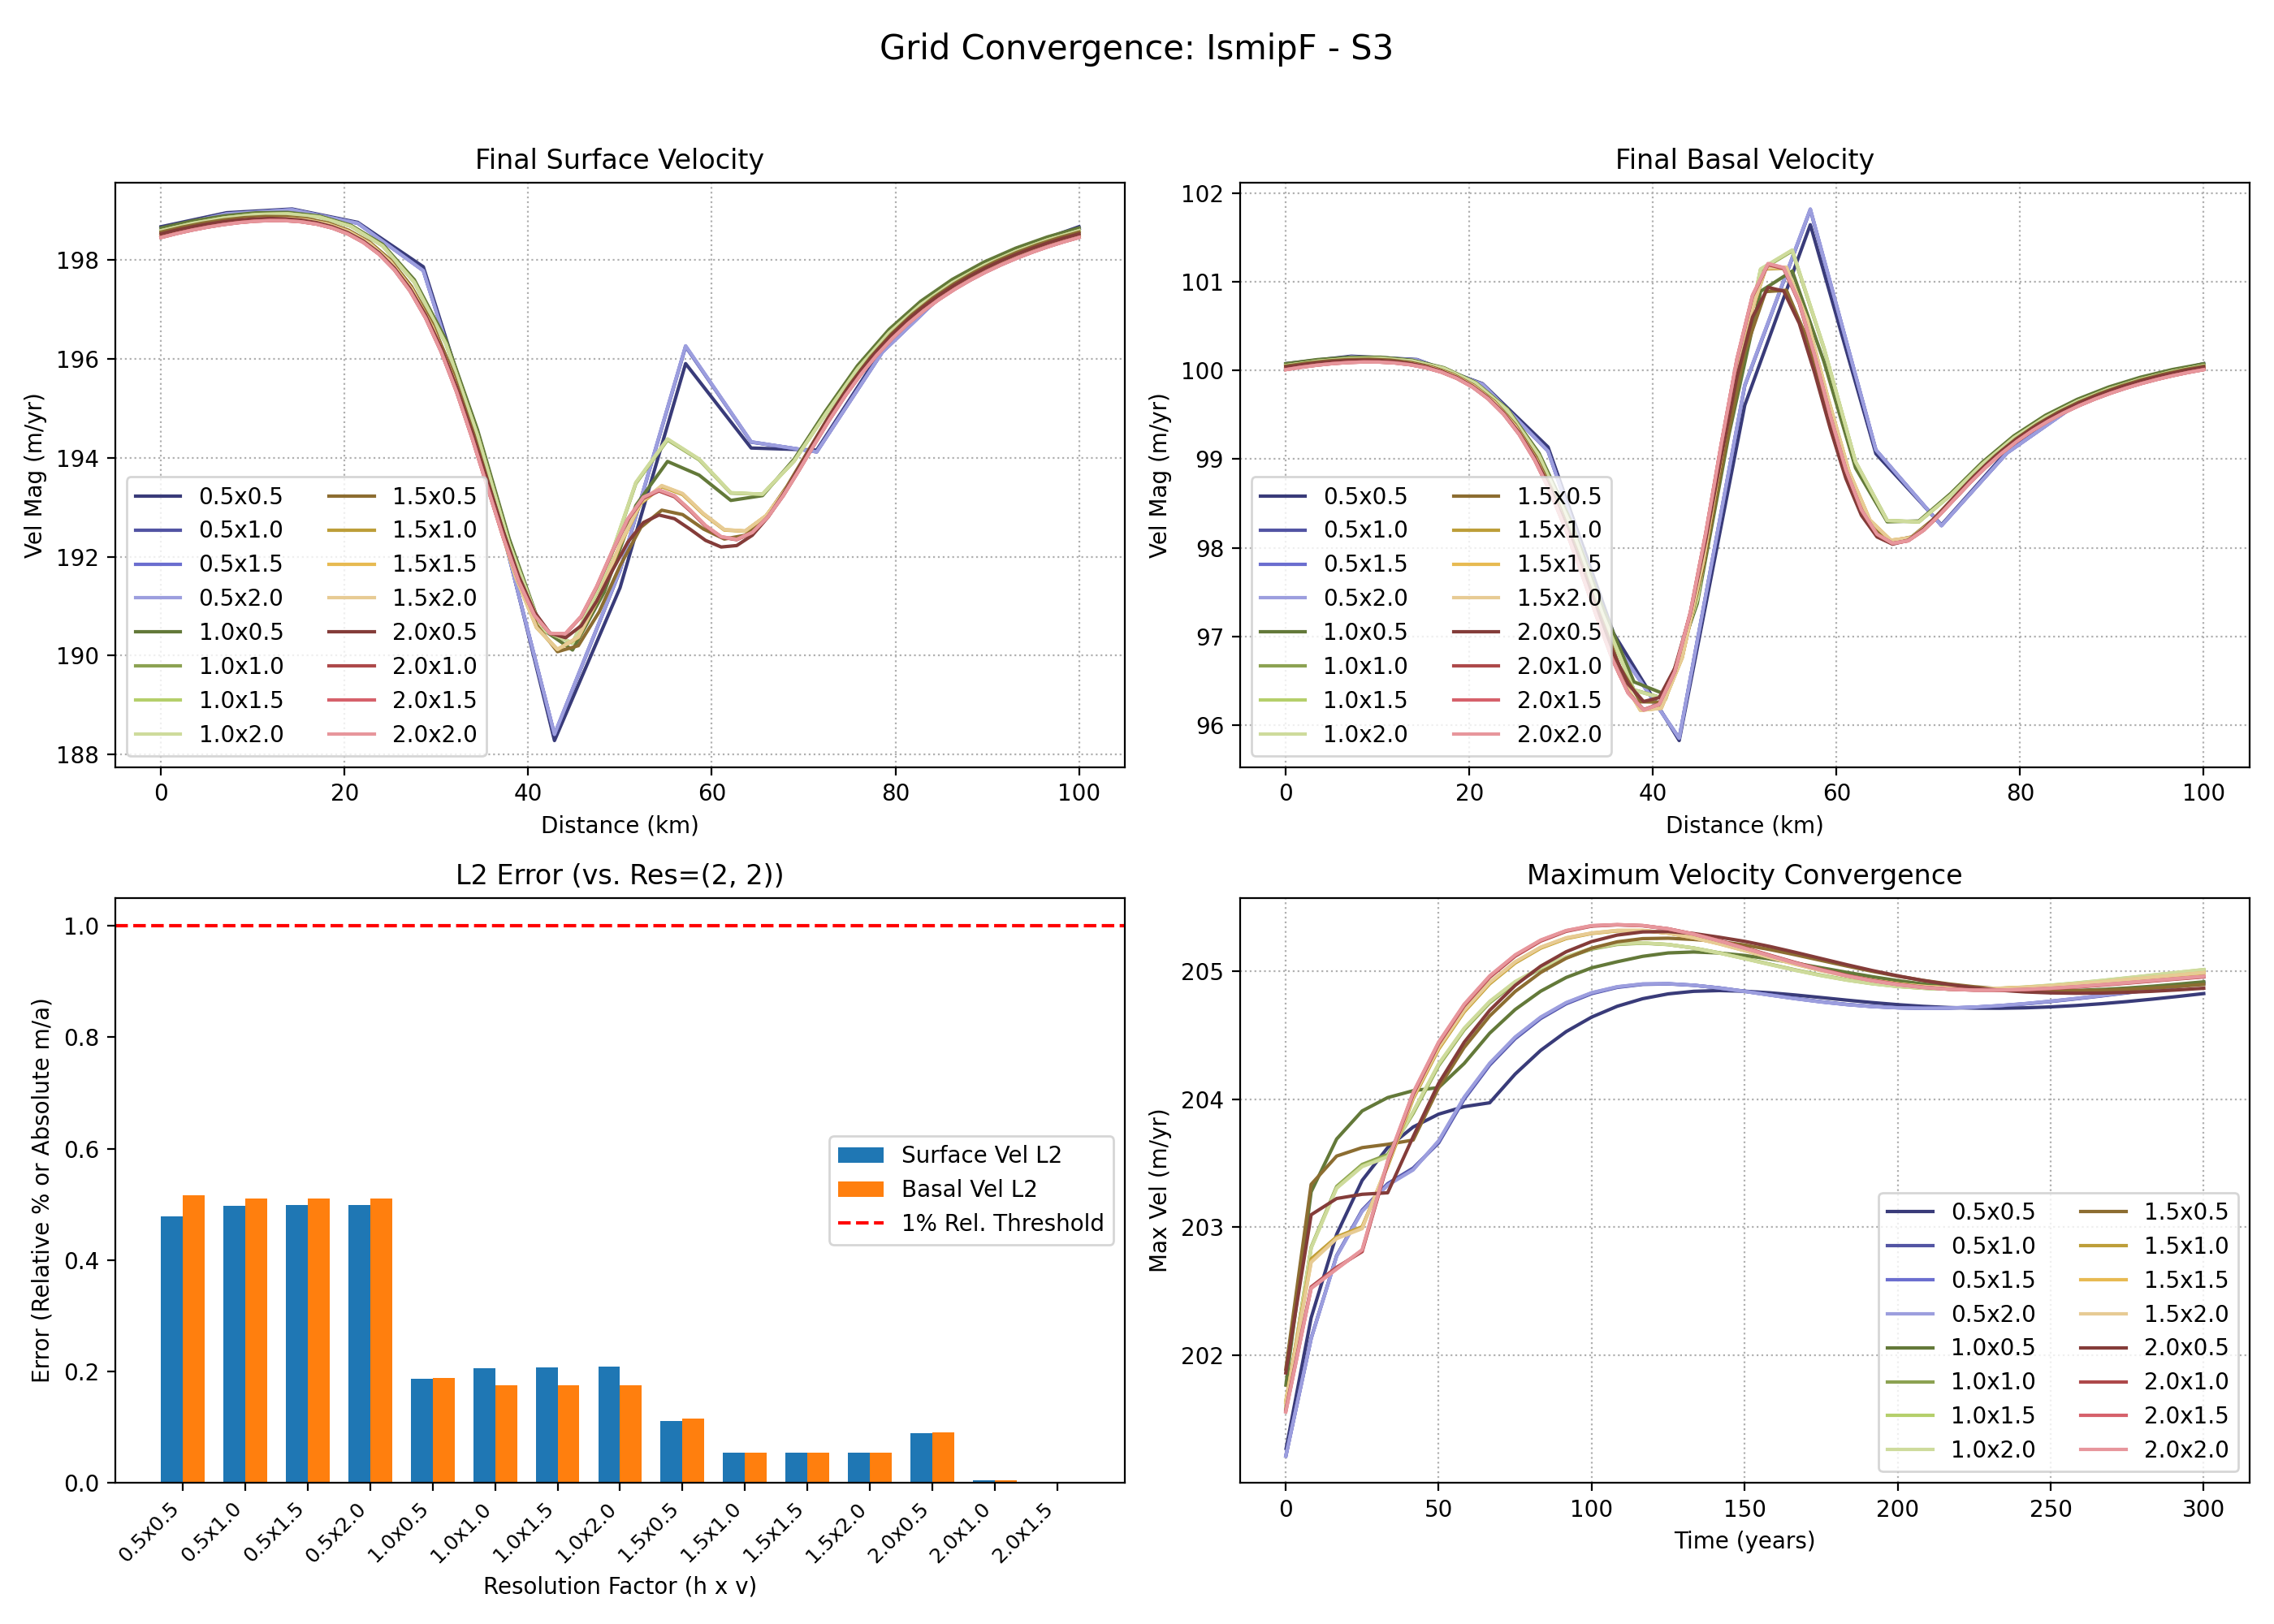
\includegraphics[scale=0.40]{figures/IsmipF_S3_convergence_summary.png}
    \caption{Grid convergence analysis for Scenario S3 (linear sliding, linear rheology, $n=1$). The four panels show: (top-left) final surface velocity profiles and (top-right) final basal velocity profiles for 16 different mesh resolutions; (bottom-left) the L2 relative error of each simulation compared to the highest-resolution mesh ($2.0\times2.0$), with a 1\% relative error threshold indicated by the dashed line; and (bottom-right) the evolution of the maximum velocity over the 300-year simulation period}
    \label{fig:grid_conv_S3}
\end{figure}
\begin{figure}[H]
    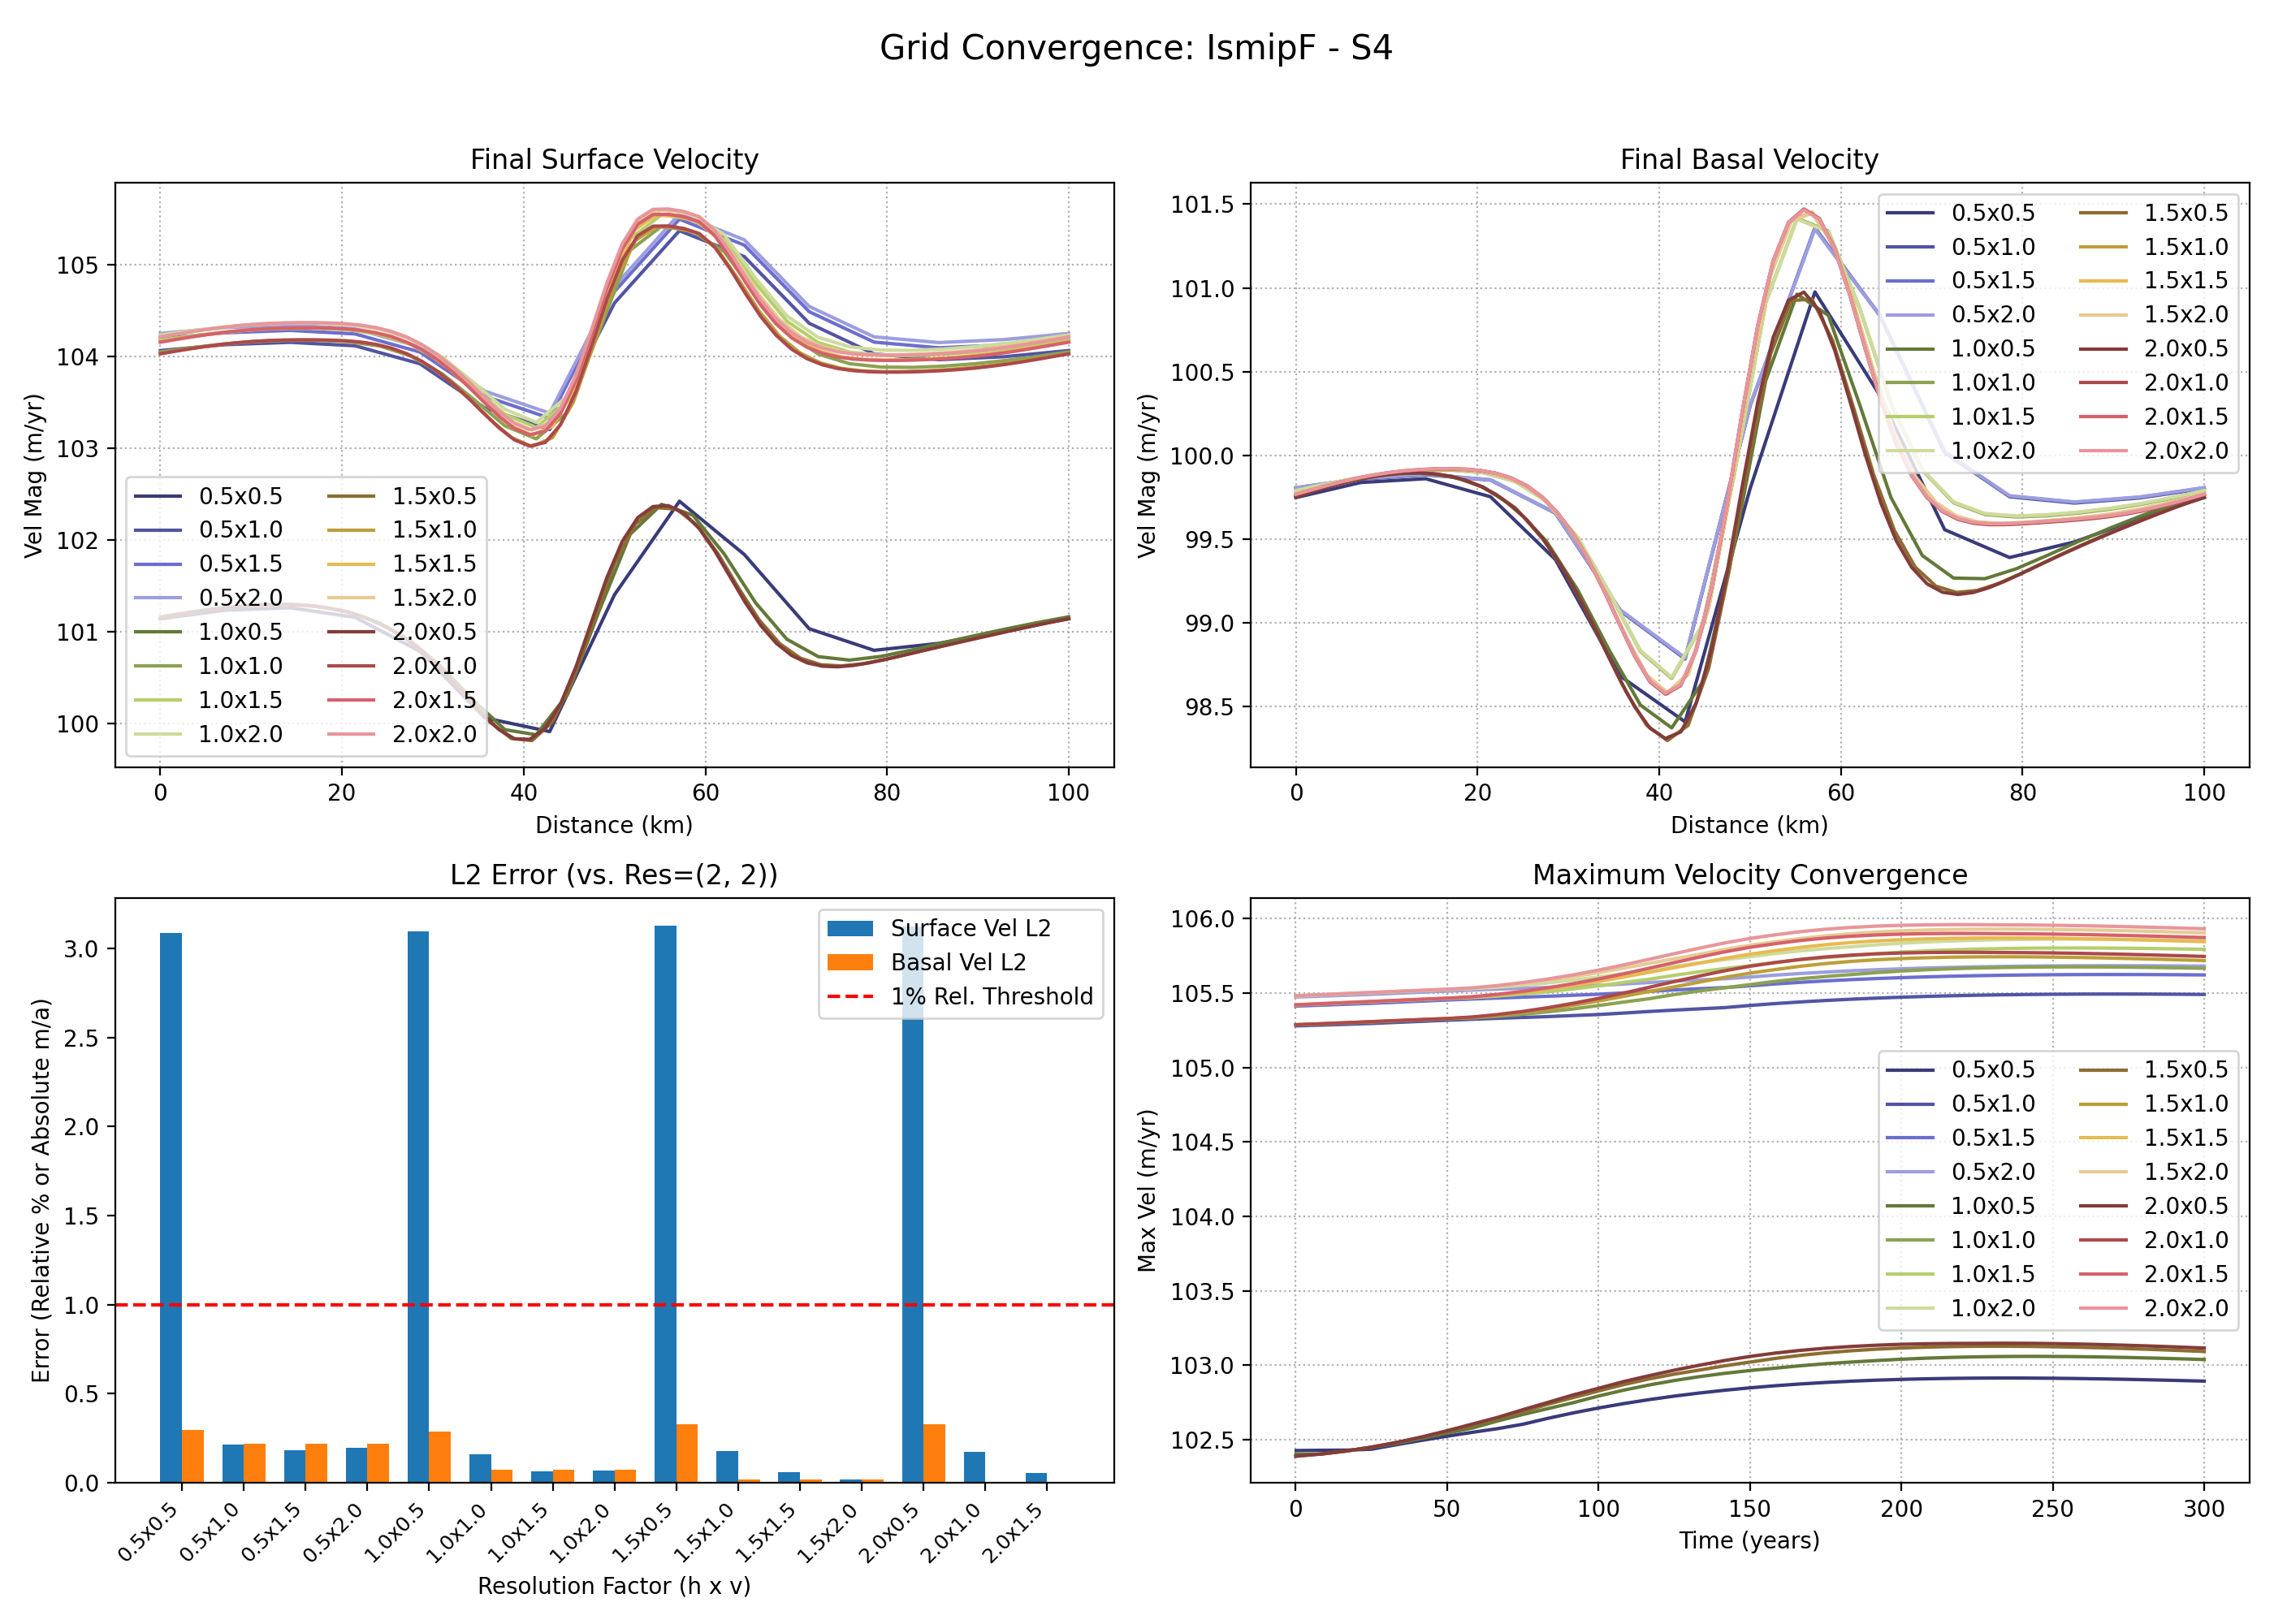
\includegraphics[scale=0.40]{figures/IsmipF_S4_convergence_summary.png}
    \caption{Grid convergence analysis for Scenario S4 (linear sliding, non-linear rheology, $n=4$). Another extension of ISMIP-HOM Experiment F, similarly to the other non-linear case (S2) in Figure~\ref{fig:grid_conv_S2}, this scenario is highly sensitive to vertical resolution. The convergence analysis shows that the 1\% relative error threshold is only achieved for simulations using the highest vertical resolution factor (2.0)}
    \label{fig:grid_conv_S4}
\end{figure}
Diagnostic convergence analyses show that the simulations are most sensitive to vertical resolution refinement. The effect is more dramatic with the non-linear rheology scenarios in Figures~\ref{fig:grid_conv_S2} and~\ref{fig:grid_conv_S4}. The convergence threshold of 1\% is only achieved for both S2 and S4 with the vertical resolution factor $2.0$. The vertical resolution of the mesh produces qualitatively different results as it is refined.
The next phase of this analysis will involve applying this validated framework to a suite of more complex and statistically realistic synthetic bedrock topographies—closely mimicking the conditions found in Antarctica—in order to further inform the development of the BedSAT inversion method. Presently, I am working on understanding the Bedmap3 and REMA digital elevation models (DEM) to develop the parameterisation of this realistic bedrock database.


% % ======================================================

% \subsubsection{Transient Analysis}
% % \begin{figure}[H]
% %     \includegraphics[scale=0.45]{figures/}
% %     \caption{}
% %     \label{fig:Transient_analysis}
% % \end{figure}
